% !TeX root = ../thuthesis-example.tex

% \chapter{异常检测算法分析与对比}
\section{开源数据集介绍}
% \subsection{UNSW-NB15}
流量异常检测领域的开源数据集要么过于久远,无法反映当前的网络环境,要么模拟访问环境过于简单,可信度很低。因此流量异常检测领域的高质量的开源数据集很少。本文采用目前应用最为广泛的两个数据集,UNSW-NB15 和 CICIDS2017,尽管这两个数据集也有很多不足。

澳大利亚网络安全中心(ACCS)的网络范围实验室在 KDD99 数据集的基础上,生成了 UNSW-NB15 数据集\cite{moustafa2015unsw} 的原始网络流量数据。UNSW-NB15利用的主要工具是 IXIA PerfectStorm,期望是可以体现网络在实际状况当中所呈现的流量。相比于陈旧的KDD99数据集\cite{ozgur2016review},其更能代表真实的网络流量。

第二个数据集CICIDS2017则是由加拿大网络安全研究所(Canadian Institute for Cyber-security)提供。与UNSW-NB15类似,CICIDS2017也是在仿真环境中模拟正常流量和攻击流量生成的。

UNSW-NB15的实验环境划分了3个子网,采用了45个独立的ip地址,持续约30个小时,采集了共100GB的原始网络流量数据。CICIDS2017的实验环境划分了2个子网,分为受害者子网和攻击者子网,受害者子网共有12台主机,攻击者子网共4台主机,累计测量时间持续约5天,共采集了51.1GB的pcap流量数据。由这两者的实验环境可以看出,开源数据集在规模上远远无法和真实流量环境对比。

% 该数据集包括 100GB的.pcap 格式的原始网络流量,具有九种攻击类型,分别是Fuzzers,Analysis,Backdoors,DoS,Exploits,Generic,Reconnaissance,Shellcode和Worms。每种攻击的具体描述和类别数目如表所示。该数据集还包含4个经过特征提取的csv文件,一共2540044 条数据。


% UNSW-NB15 数据集一共包含 47 个特征,其中时间戳,IP 地址,端口号等特征对训练无用,因此有效的特征一共 41 个。 
% 下面对这些特征做一个概括的说明。按照数据集作者的思路,可以分为基本
% 特征,内容特征,时间特征和额外生成的特征这几类。

以UNSW-NB15为例,图\ref{fig:UNSW-NB15数据集生成过程}展示了该数据集的生成过程。首先,通过使用Tcupdump工具监测仿真环境中的流量情况,生成pcap文件;然后使用Argus\footnote{https://qosient.com/argus/index.shtml}和Bro-IDS\footnote{https://www.bro.org/index.html}工具从报文信息中直接提取基于数据包和数据流的特征,并根据五元组(源/目的ip地址,源/目的端口号,协议类型)信息进行匹配,此时基本特征、内容特征和时间特征已生成;接下来为了能够更有效地识别攻击,还需要额外生成一些统计特征。最终将这些特征保存成csv文件。



这些数据集生成流程和特征提取方法给后续我们分析清华大学校园网的流量数据提供了参考。


\begin{figure}
    \centering
    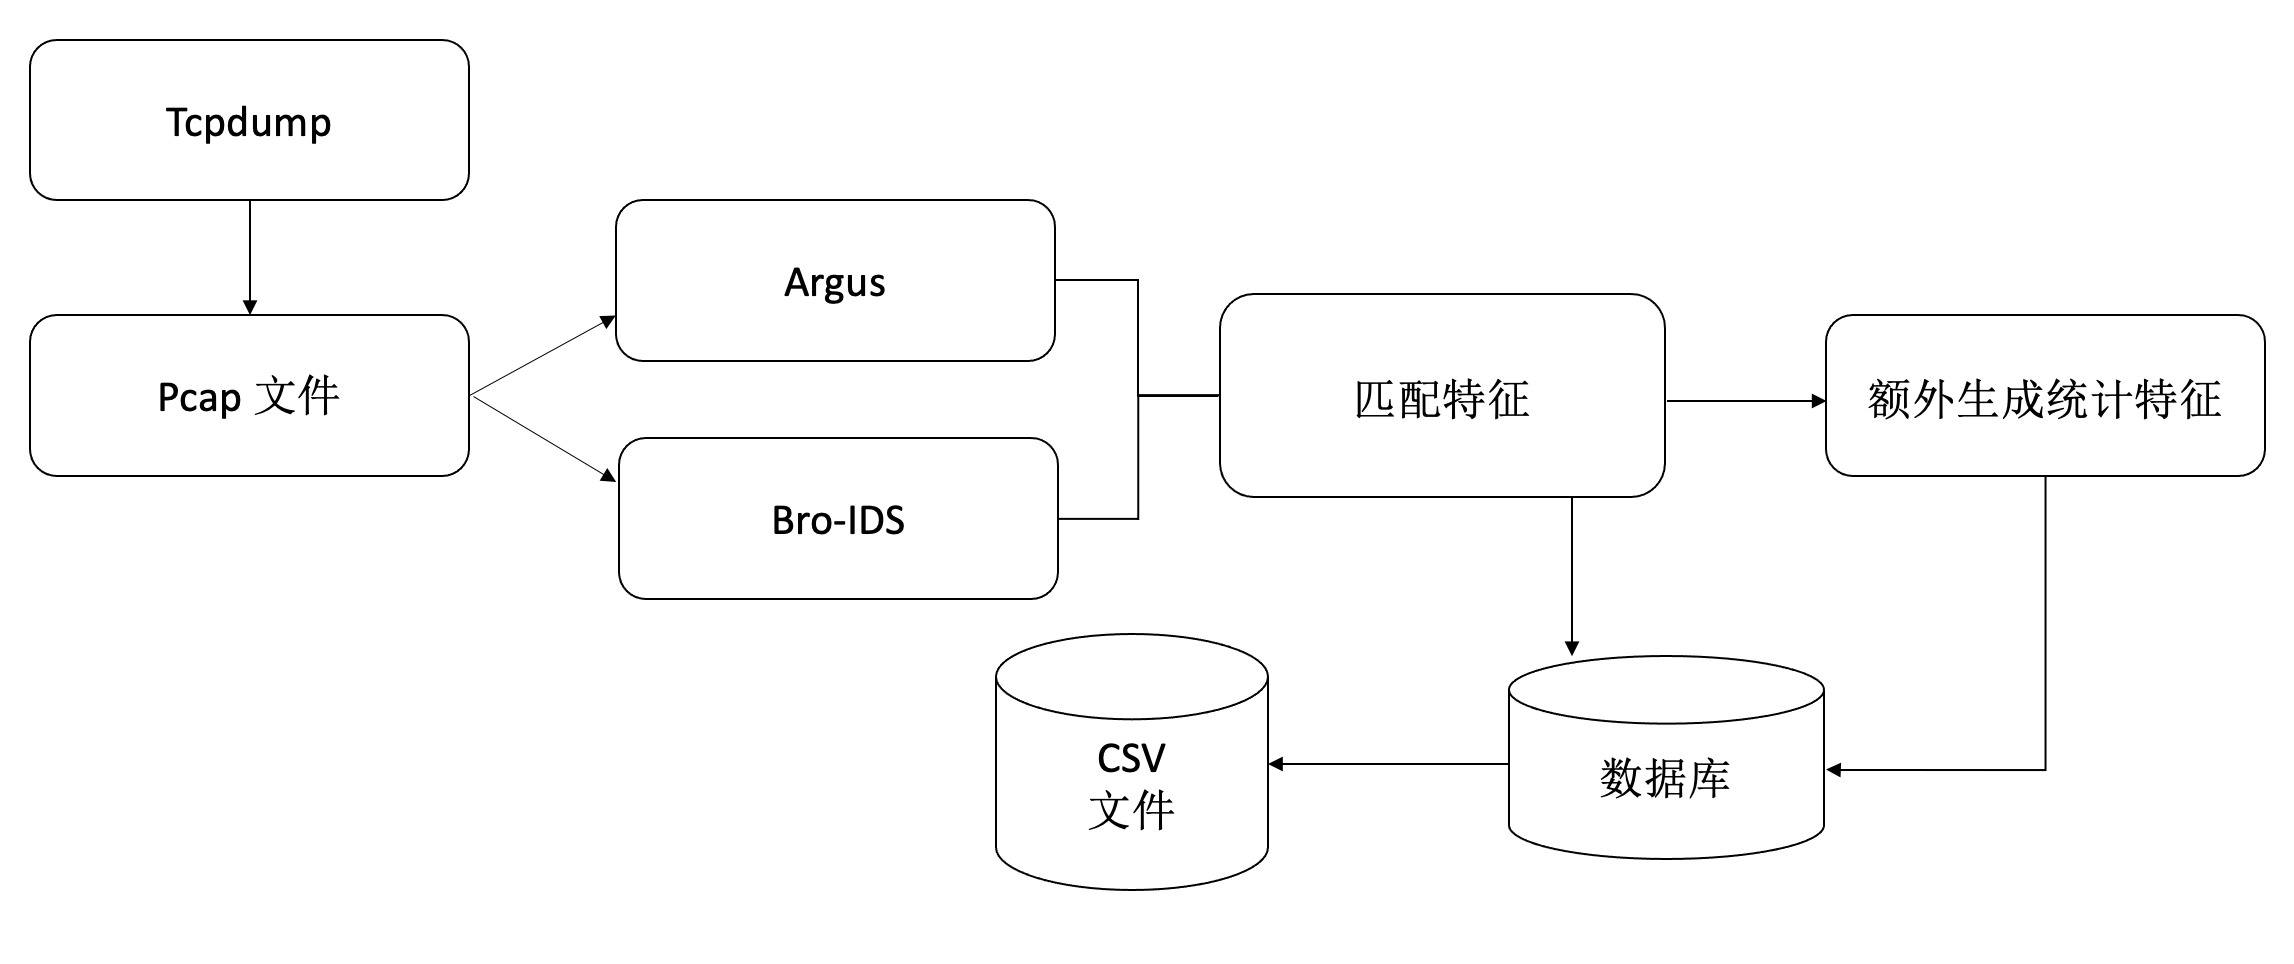
\includegraphics[width=0.6\linewidth]{UNSW-NB15 framework.png}
    \caption{UNSW-NB15数据集生成过程}
    \label{fig:UNSW-NB15数据集生成过程}
  \end{figure}


\section{校园网数据集介绍}
清华大学无线网规模巨大,具有超过6万名日活跃用户,13万个可用ip地址,是全球最大的校园无线网之一。通过出口网关的服务器我们可以得到海量的真实流量数据,但是这与可进行分析和训练的数据集之间还有巨大的鸿沟。因此本节参考图\ref{fig:UNSW-NB15数据集生成过程}中的数据集生成流程,结合UNSW-NB15和CICIDS2017两个数据集中特征的特点,生成了校园网的特征数据集。校园网数据集制作流程如图\ref{fig:流量数据集制作流程}所示。首先将pcap流量数据切分成多个会话(session,双向流中所有的数据包),依次从每个会话中提取报文信息以及统计信息构成特征;然后以五元组作为流的标识符,把从SOC平台中得到的告警信息与特征信息合并起来,就生成了最终的数据集。将该数据集命名为CAMPUS数据集。
\begin{figure}
    \centering
    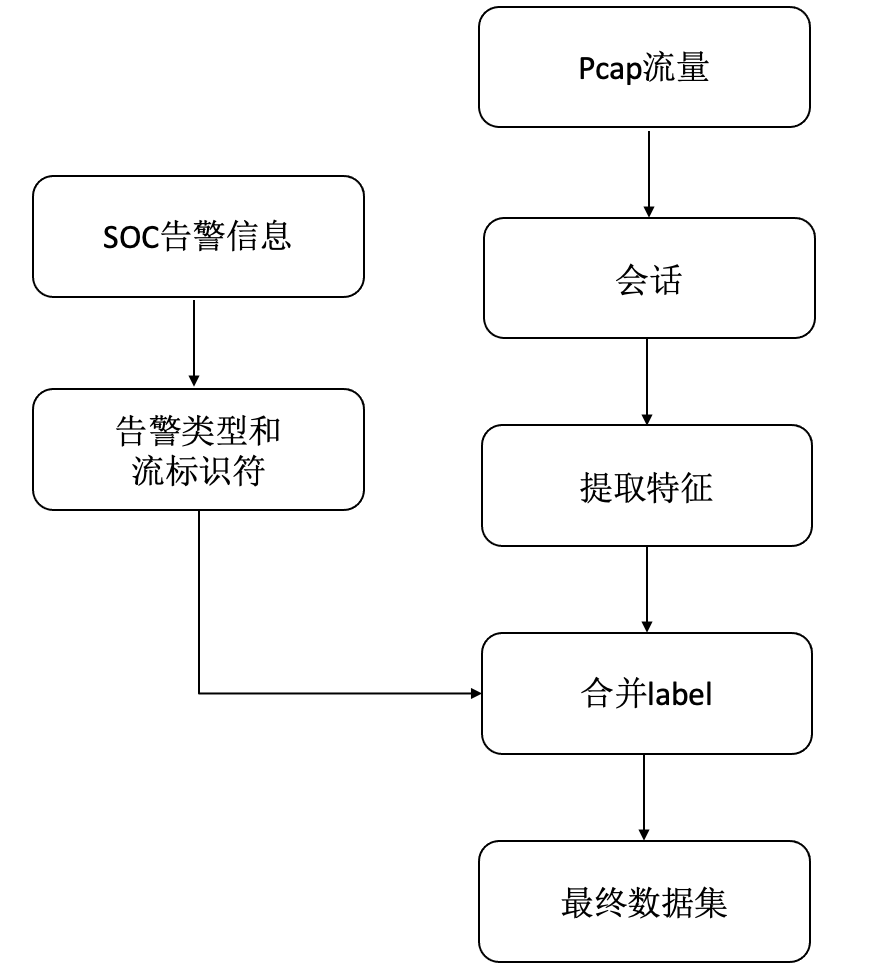
\includegraphics[scale=0.6]{校园网数据集制作流程.png}

    \caption{校园网流量数据集制作流程}
    \label{fig:流量数据集制作流程}
  \end{figure}

在本文的实验中,我们采集了三段共约25小时的数据,第一段从2021年3月19日8点43分采集到2021年3月19日12点08分,持续3.5小时,共420GB大小,用于验证特征提取算法以及经典模型的实验对比,第二段从2021年3月19日13点06分采集到2021年3月20日6点52分,持续18小时,共1100GB大小,用于分析特征关系图的有效性以及训练FG-RNN算法,第三段从2021年3月20日14点26分采集到2021年3月20日18点21分,持续4小时,共350GB大小,用于验证FG-RNN算法的鲁棒性。
% 三段分别持续3.5小时、18小时、4小时,每段大小为420GB、1100GB、350GB。

以上数据为出口网关处的全流量数据,此外我们还利用了安全管理平台(Security Operations Center,SOC)的威胁告警日志,
接下来分别介绍这两类数据。

\subsection{全流量日志数据}
校园网的原始数据为抓包(Packet Capture,pcap)流量,如下图~\ref{fig:wireshark}所示,其中包含每个数据包的详细信息,如五元组、报文头部信息、报文内容等。清华大学校园网共有6个B的地址资源,由于本实验的计算和存储资源的限制,我们只采集了一个B类地址的流量数据,最多可容纳6万台主机,相比于开源数据集采集环境的数十台主机,本数据集规模可谓宏大。

另外,本文对所有用户隐私信息(如IP地址和MAC地址,报文中的明文信息等)都进行了匿名化处理,保证不会泄露用户的任何隐私信息。

\begin{figure}
    \centering
    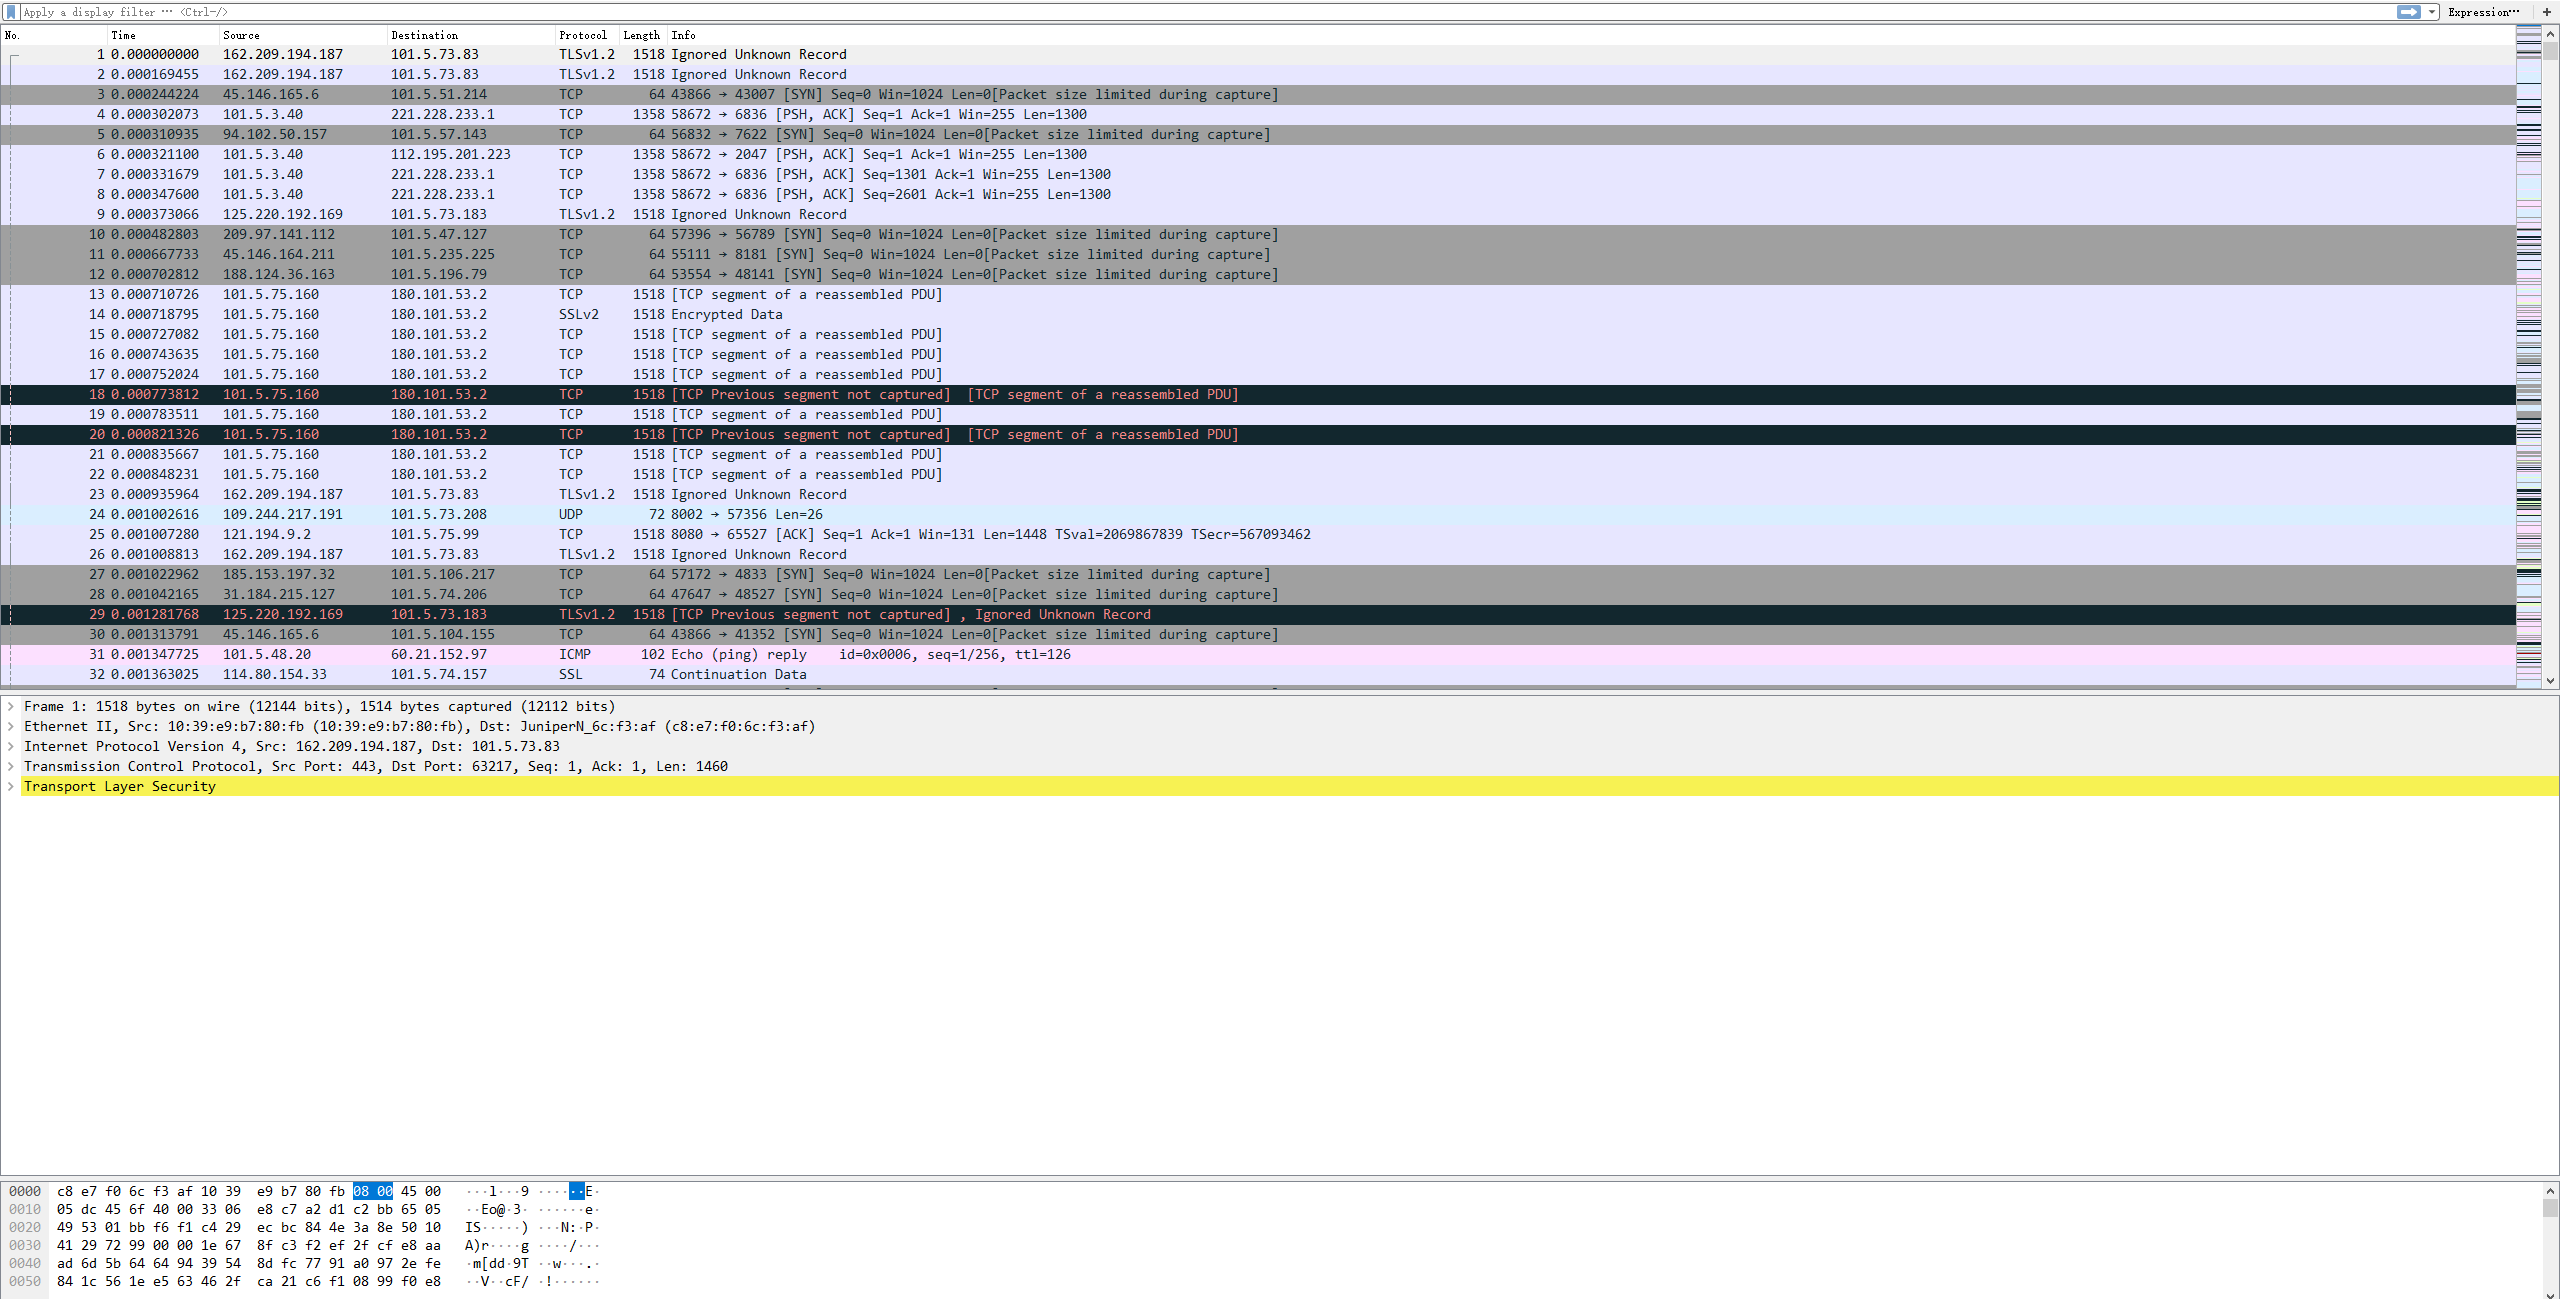
\includegraphics[scale=0.22]{wireshark流量图.png}
    \caption{流量数据示意图}
    \label{fig:wireshark}
  \end{figure}

全流量数据宏观上看具有周期性,例如图\ref{fig:用户流量变化图}表示每秒钟报文数量的变化。但是由于我们是基于每条流的信息进行异常检测,平均每秒钟数百万的报文信息之间大多毫无关联,因此仅需从流的视角对全流量数据进行特征提取。本文采用了CICFlowMeter\footnote{https://github.com/ahlashkari/CICFlowMeter}工具,其大致原理为从pcap文件中依次读取报文(packet),判断当前报文是否属于当前统计的所有流中,若存在则更新该流的统计特征信息,否则创建一条新的流,直至遇到包含FIN标志的报文或者超时。最后将得到的每条流的特征信息依次打印到csv文件中。
%   对于机器学习模型来说,通常
%   不是直接对原始的流量进行检测,而是通过对流量提取特征,得到样本的特征向
%   量后进行检测和分类。


\subsection{威胁告警日志}
我们通过全流量日志得到了特征数据集,但是由于缺乏标注,该数据集无法进行训练以及验证。因此为了得到可进行训练的有效数据集,我们还需要对特征数据集添加标注。我们根据现有的SOC平台得到标注数据,然后进行数据清洗、数据预处理等步骤。图\ref{fig:NOC平台数据样例}为SOC平台的数据样例。
\begin{figure}
    \centering
    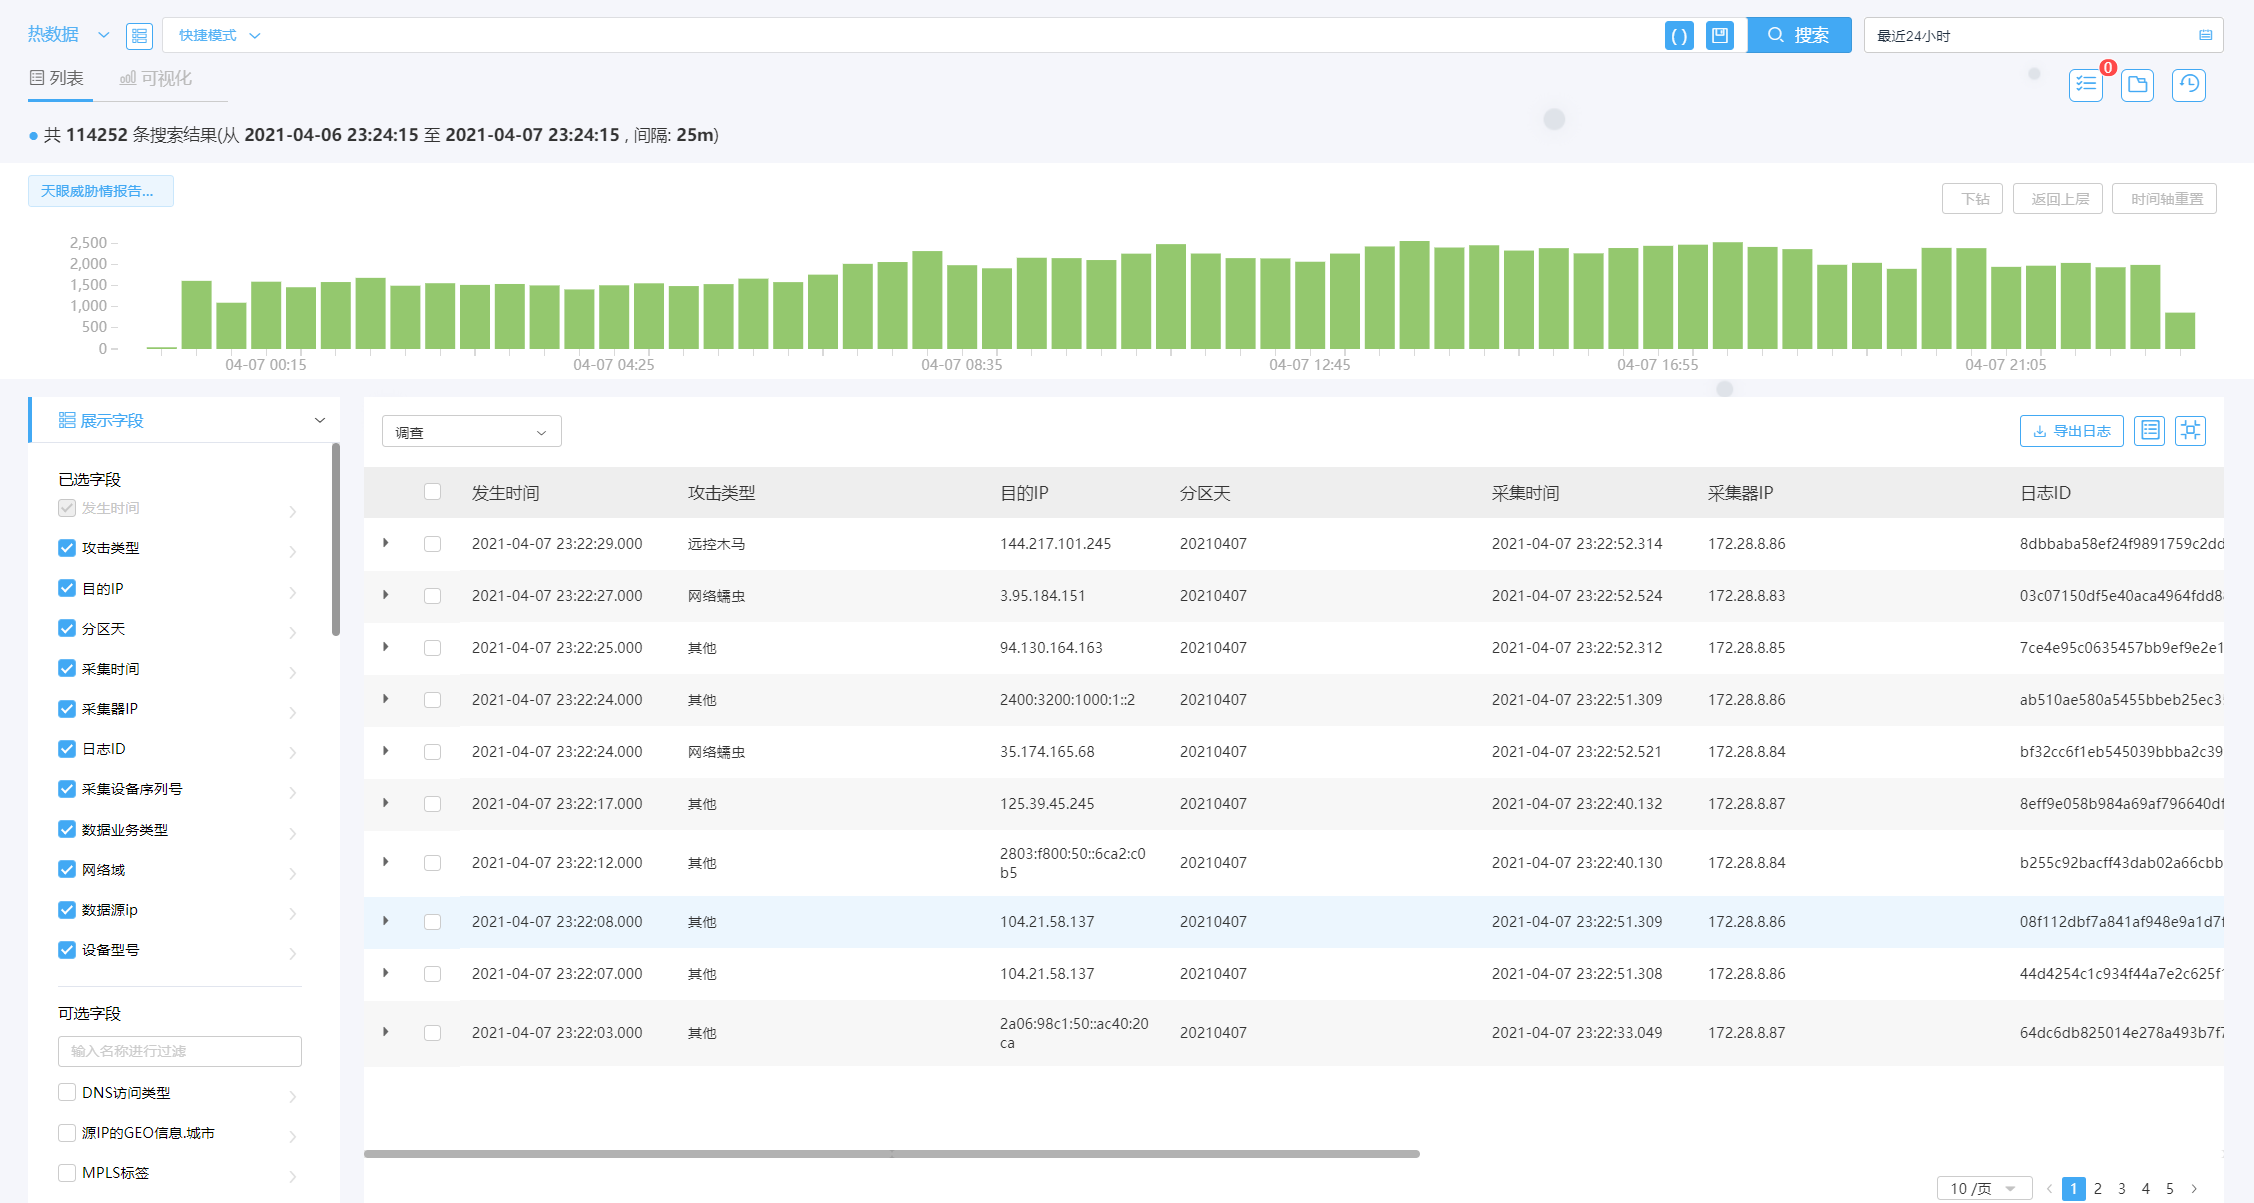
\includegraphics[scale=0.35]{NOC平台.png}
    \caption{SOC平台数据样例}
    \label{fig:NOC平台数据样例}
  \end{figure}


图\ref{fig:告警趋势图}为SOC平台给出的一个月内告警信息的趋势图。从图中可以看出,告警信息大致稳定在每天9000个,存在极端情况。
% 图\ref{fig:告警分布}为告警类型的分布,从中可以看出,远控木马、暴力猜解、后门程序为主要的攻击手段。
\begin{figure}
    \centering
    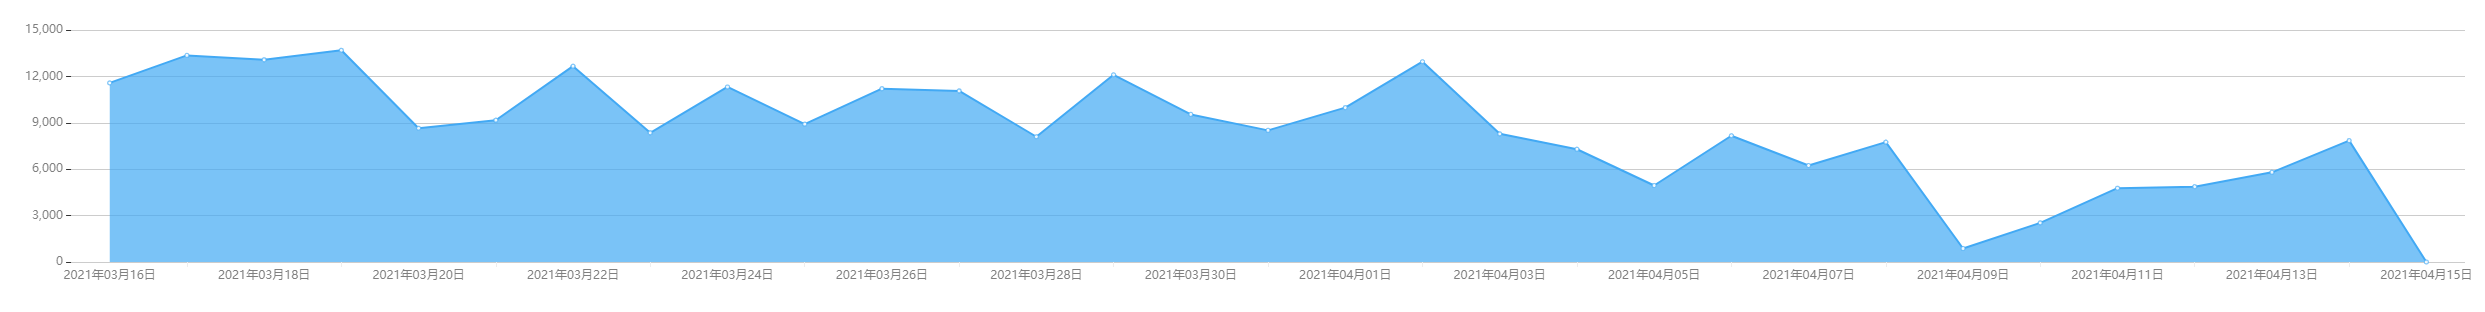
\includegraphics[scale=0.15]{告警趋势图_20214150748.png}
    \caption{告警趋势图}
    \label{fig:告警趋势图}
  \end{figure}
  % \begin{figure}
  %   \centering
  %   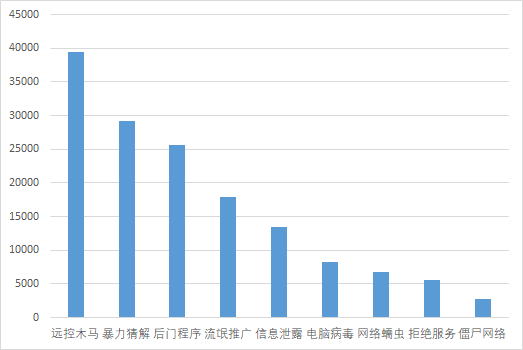
\includegraphics[scale=0.6]{告警分布.png}
  %   \caption{告警分布}
  %   \label{fig:告警分布}
  % \end{figure}
\section{两类数据集对比}
在对两大类数据集进行异常检测的算法验证之前,我们首先从数据规模和异常种类两方面对其进行了对比,以便对CAMPUS数据集有一个直观的印象。

表\ref{数据集规模对比}是三种数据集在规模上的对比,从中可以看出,CAMPUS数据集规模宏大,子网内ip数量和使用的流量文件大小是开源数据集的百倍甚至千倍,并且CAMPUS中异常种类也要比开源数据集更多。
\begin{table*}[h]
  \small
  \caption{数据集规模对比}
  \label{数据集规模对比}
  \centering
  \begin{tabular}{c|cccc}
  \toprule
  
   数据集名称 &  独立ip数量  & 采集时长 &  流量文件(pcap)大小 & 异常种类 \\
  \midrule
  
  UNSW-NB15 & 45 & 30h & 100G & 9   \\ 
  CICIDS2017 & 16 & 5天 & 51G & 4 \\
  CAMPUS & 数万 & 25h & 2T & 10多种\\
 
   \bottomrule
  
  \end{tabular}
  \end{table*}

图\ref{fig:数据集异常类别对比}展示了三种数据集在异常类别上的对比,可以看出CICIDS2017数据集中的异常大部分是拒绝服务和端口扫描,分别占比约70\%和28\%,其中包括多种子类型,例如慢速连接攻击、SYN泛洪攻击、黑市工具等;而UNSW-NB15数据集约67\%的异常是暴力猜解;CAMPUS1和CAMPUS2分别是CAMPUS数据集的两个时间切片,异常的种类比开源数据集更加丰富。并且尽管它们同属于一个数据集,但是由于处于不同的时间窗口内,异常种类的占比差异很大。而反观开源数据集,由于全部流量都是人工生成,其异常种类和占比都是固定不变的。这种异常种类的动态性给我们的异常检测算法带来了挑战,因此算法的适应性需要足够强,面对复杂的流量环境依然可以有效地检测出异常。

  \begin{figure}
    \centering
    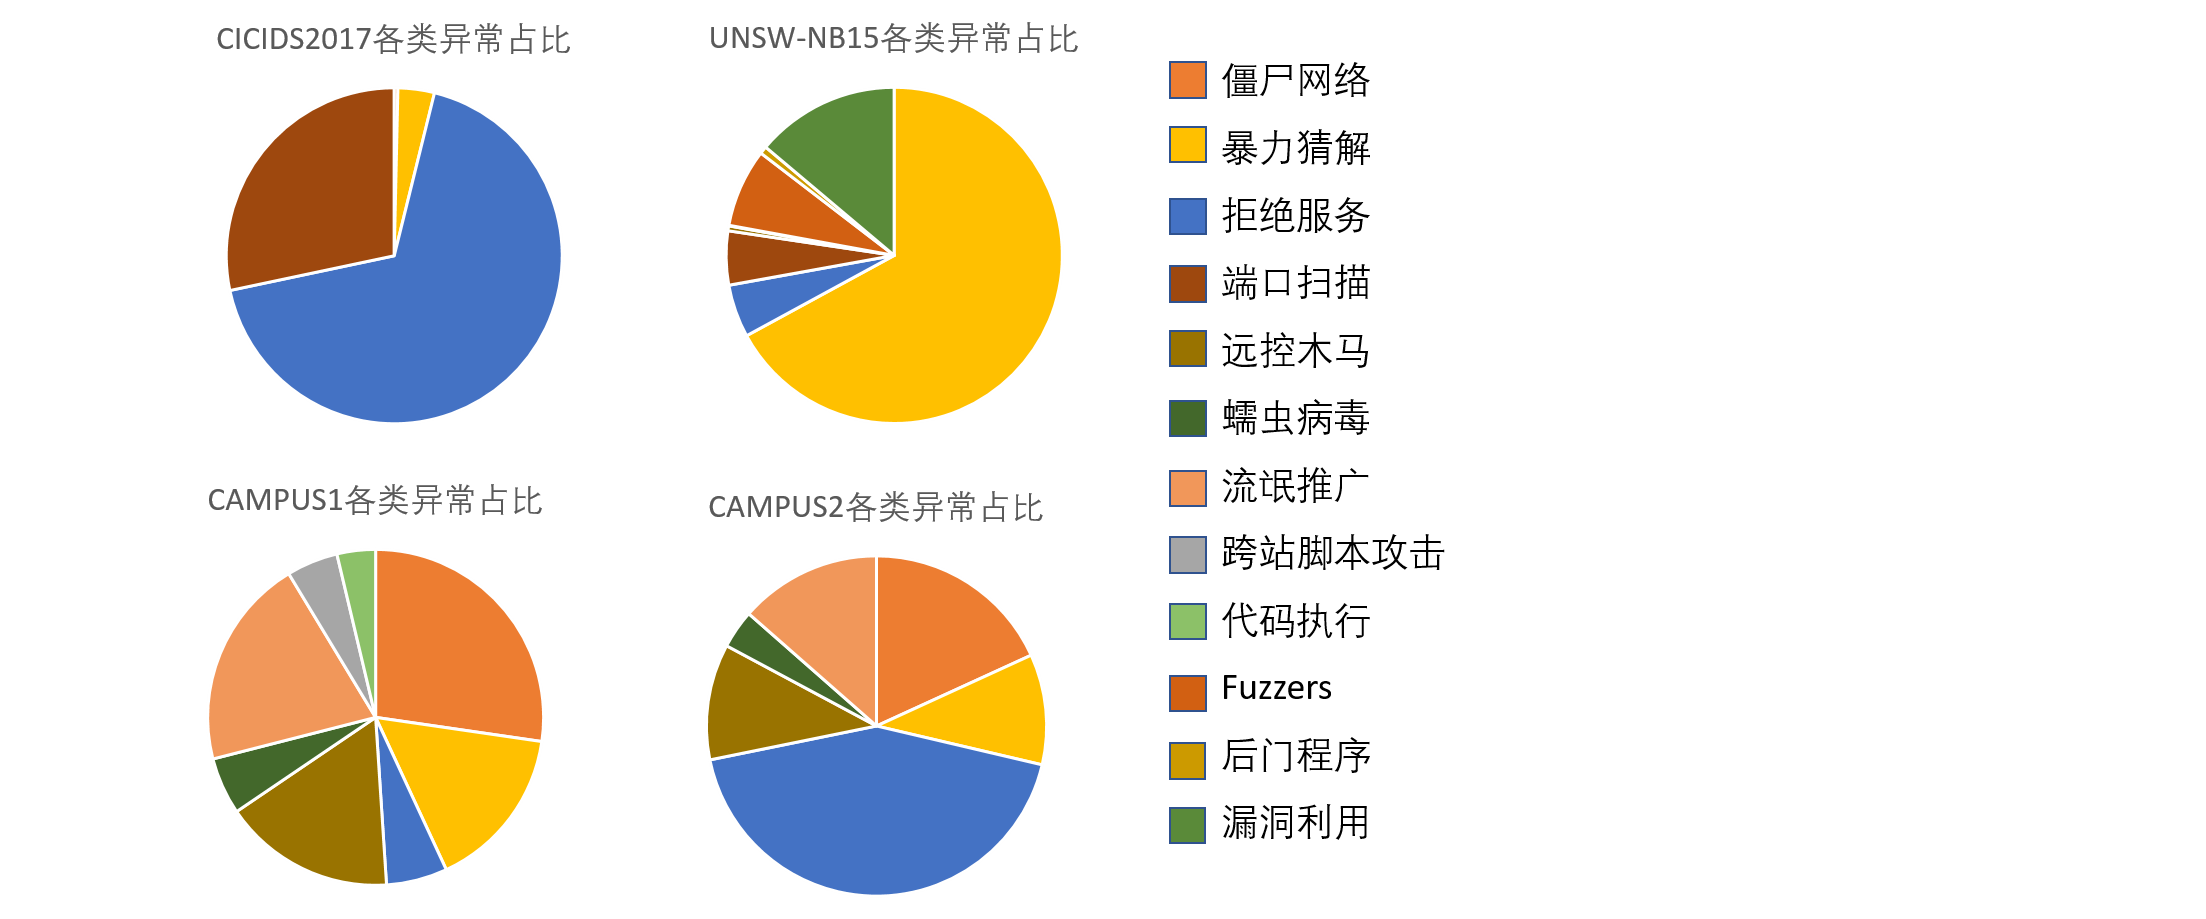
\includegraphics[scale=0.5]{数据集异常类别对比}
    \caption{数据集异常类别对比}
    \label{fig:数据集异常类别对比}
  \end{figure}

% \section{评价指标}
% 在实验中,本论文使用四个指标来评估模型的性能:准确率,精确度,召回
% 率和 $F1-score$。对于一个数据样本检测的结果可分为下面的结果:

% \begin{enumerate}
%     \item TP:入侵网络流量被入侵检测正确的识别为入侵网络流量。
%     \item TN:正常网络流量被入侵检测正确的识别为正常网络流量。
%     \item FN:入侵网络流量被入侵检测错误的识别为正常网络流量。
%     \item FP:正常网络流量被入侵检测错误的识别成入侵网络流量。
% \end{enumerate}

% % 1. TP:入侵网络流量被入侵检测正确的识别为入侵网络流量

% % 2. TN:正常网络流量被入侵检测正确的识别为正常网络流量

% % 3. FN:入侵网络流量被入侵检测错误的识别为正常网络流量

% % 4. FP:正常网络流量被入侵检测错误的识别成入侵网络流量

% 论文使用下面的方法去评估我们提出方法的性能:
% 准确率(Accuracy): 预测正确的样本的数量与所有被预测样本数量的比值,
% 公式如下 所示。
% \begin{equation}
%     Accuracy = \frac{TP + TN}{TP + TN + FN + FP}
% \end{equation}

% 精确度(Precision): 这个指标于分类器衡量的被错误分类的数量所惩罚的
% 正确分类的数量,公式如 下所示:
% \begin{equation}
%     Precision = \frac{TP}{TP + FP}
% \end{equation}
% 召回率(Recall): 针对样本而言的表示的是数据正样本中有多少被预测正
% 确。这种度量反映了分类器检测网络攻击的能力,公式如下  所示:
% \begin{equation}
%     Recall = \frac{TP}{TP+ FN}
% \end{equation}
% $F1-score$:此调和平均值这是用以计量精确度以及召回率的,可以平衡的反映算法的精确度,公式如下所示:
% \begin{equation}
%     F1-score = 2*\frac{Precision * Recall}{Precision + Recall}
% \end{equation}
\section{现有算法在不同数据集上的对比}
本文利用sklearn、pytorch等Python库分别实现了“逻辑回归(LR)”、“决策树”(DT)、“随机森林(RF)”、标准的“循环神经网络”(RNN)、“长短期记忆网络”(LSTM)、“门控循环单元”(GRU)几个模型。

本节分别在以上三个数据集上进行实验,对比了以上6个经典模型,表\ref{不同数据集下实验评估结果}是评估结果,评估指标为正样本的准确率,其中多分类任务的准确率指标为对于每个标签,分别计算precision,然后取不加权平均值。由表中可以看出,在两个开源数据集上,各个算法在二分类任务(即仅需检测是否发生异常)的效果相差不大,在多分类任务(即需要判断异常类型)里,神经网络类的模型效果均要略好于基于分类的机器学习模型。这说明针对模拟仿真出的有规律的流量数据,各类算法可以有效地学习出正常流量的基线,而不同类型的异常具有各自的特征,各个算法的能力在学习这些特征的过程中显现出差异。但是这些算法在CAMPUS数据集上表现很差,甚至和随机猜测的效果差不多。说明现有的算法无法应对复杂的清华大学校园网流量环境,需要我们进一步对这些算法进行优化,以适应校园网流量环境。因此,接下来我们以DT和RF模型作为baseline,对RNN类算法进行特征分析,找到其表现不佳的原因,并且做出改进。




\begin{table*}[h]
    \small
    \caption{不同数据集下实验评估结果(\%)}
    \label{不同数据集下实验评估结果}
    \centering
    \begin{tabular}{c|c|ccc|ccc}
    \toprule
    
     数据集 &  任务  &  
     LR &  DT & RF & RNN & LSTM & GRU  \\
    \midrule
    
    UNSW-NB15 & 二分类 & 96.8 & 97.33 & 98.52 &  95.51 & 96.74 & 94.91  \\ 
    
    & 多分类 &90.73 & 91.36 & 91.82 & 93.98 & 92.11 & 92.30  \\
    
    \midrule
    CICIDS2017 & 二分类 & 98.26 & 97.11 & 95.54 & 90.18 & 88.04 & 91.49  \\
    & 多分类 & 91.01 & 92.37 & 94.41 & 92.31 & 93.16 & 94.18 \\
    \midrule
    CAMPUS & 二分类 & 76.98 & 77.95 & 77.51 & 55.62 & 59.80 & 55.25 \\
    & 多分类 & 73.33 & 74.01 & 74.54 & 53.01 & 56.59 & 59.28 \\
   
     \bottomrule
    
    \end{tabular}
    \end{table*}


\section{现有算法存在的问题}
截至目前, 异常检测算法的种类已经不可胜数,其中所使用的原理都有差别,针对的领域也各异,流量特征自然也不一样。但通过本文的分析我们可以看出,在应对校园网大规模、应用类型多、异常流量是常态且多种异常相互叠加的场景下,现有异常检测算法大多仍存在以下缺陷:

\begin{enumerate}
  % \item 面对海量数据规模时,无法或很难做到实时性;
  \item 应用类型多导致流量特征复杂,因此很难达到较高的检测率和较低的误报率;
  \item 不管是传统机器学习算法还是拟合能力更强的深度学习模型,都很难有效地从复杂的流量环境中学习到正常流量的基线;
  \item 面对海量数据规模时,现有的算法模型无法或很难做到实时性。
\end{enumerate}

根据以上几点缺点,本文后续章节提出了一种基于特征关系图的神经网络算法,并且在此基础上实现了一个流量异常检测系统。

\section{本章小结}
% 本章是相关工作,首先介绍了网络流量异常的定义和分类,然后按照不同的类别综述了网络流量异常检测的常用算法,最后介绍了循环神经网络的相关原理。
本章首先对网络流量异常检测领域的相关工作进行了综述,然后介绍了常用的异常检测数据集和本文中使用的校园网数据集,最后在多个数据集上对异常检测算法进行了分析与对比。

% \section{本章小结}
% 本章对本文使用的三种数据集进行了介绍和对比,并且在这些数据集上对现有经典算法进行了评估,最后分析了现有算法存在的问题。

% \begin{table*}[h]
%   \small
%   \caption{不同数据集下实验评估结果(\%)}
%   \label{不同数据集下实验评估结果}
%   \centering
%   \begin{tabular}{c|c|ccc|ccc|c}
%   \toprule
  
%     数据集 &  任务  &  
%     LR &  DT & RF & RNN & LSTM & GRU & FG-RNN  \\
%   \midrule
  
%   UNSW-NB15 & 二分类 & 96.8 & 97.33 & 98.52 &  95.51 & 96.74 & 94.91 & 95.8 \\ 
  
%   & 多分类 &94.73 & 97.96 & 96.82 & 93.98 & 92.11 & 94.30 & 94.24 \\
  
%   \midrule
%   CICIDS2017 & 二分类 & 98.26 & 97.11 & 95.54 & 90.18 & 88.04 & 91.49 & 92.45 \\
%   & 多分类 & 97.01 & 97.37 & 94.41 & 88.31 & 91.16 & 90.18 & 90.67\\
%   \midrule
%   CAMPUS & 二分类 & 76.98 & 77.95 & 77.51 & 55.62 & 59.80 & 55.25 & 84.34 \\
%   & 多分类 & 73.33 & 74.01 & 74.54 & 53.01 & 56.59 & 59.28 & 82.74\\
  
%     \bottomrule
  
%   \end{tabular}
%   \end{table*}


% \section{两类数据集对比}



% 本节对上述两大类三种数据集从数据规模、数据特点、模型效果等方面进行了对比,并得出了以下结论:

% 1.CAMPUS数据集的规模远大于两个开源数据集;
% 2.CAMPUS数据集的异常种类分布具有动态性,不同时间窗口内各类异常的占比可能会相差很大,例如某5分钟内ACK Flooding的占比达到97\%以上,但是在另一个5分钟内其占比仅不到1\%。而由于开源数据集是人为通过脚本生成的正常流量和异常流量,其各类异常占比通常是提前设定好的。
% 3.各类模型在CAMPUS上效果不佳,

% 因此,接下来我们从特征分析的角度着手,对比各类算法,找出神经网络模型在CAMPUS数据集性能不佳的原因。


% \begin{table*}[h]
%   \small
%   \caption{参数设置(\%)}
%   \label{不同数据集下实验评估结果}
%   \centering
%   \begin{tabular}{c|c|cc}
%   \toprule
  
%     模型参数 & 实验ID & 参数值  & accuracy \\
%   \midrule
  
%       & 01 & 50& 97.33  \\ 
%   batchsize & 01 & 100&97.33  \\
%       & 01 & 200& 97.33  \\
%     \bottomrule
  
%   \end{tabular}
%   \end{table*}